\section{Cavern $\gamma$ Generator}

\par
Although the LZ detector has been constructed underground to limit cosmic radiation, it does come with a drawback of being in a mine with a non-negligibly radioactive rock and the shotcreat and gravel within the David Cavern.
The rate of this has been measured and can be attributed to the shotcreat and gravel. 
One of the most significant sources of background come not from any internal component but rather from $^{238}U$, $^{232}Th$ and $^{40}K$ decays from the cavern in which the LZ detector exists \cite{LZ_Gamma_Ray_Background_ref}.
However, this is a computationally intensive process to simulation $\gamma$'s where the majority will not reach the actual detector.
To compensate, a generator for these $\gamma$'s was created - described in XXX.
For the creation of the generator additional cavern properties are added to the simulation.
Namely; a steel pyramid and gravel beneath the water tank, and the cavern gamma. 
These adaptions are shown in Figure \ref{fig:Cavern_Geometry}.

\begin{figure}[!htbp]
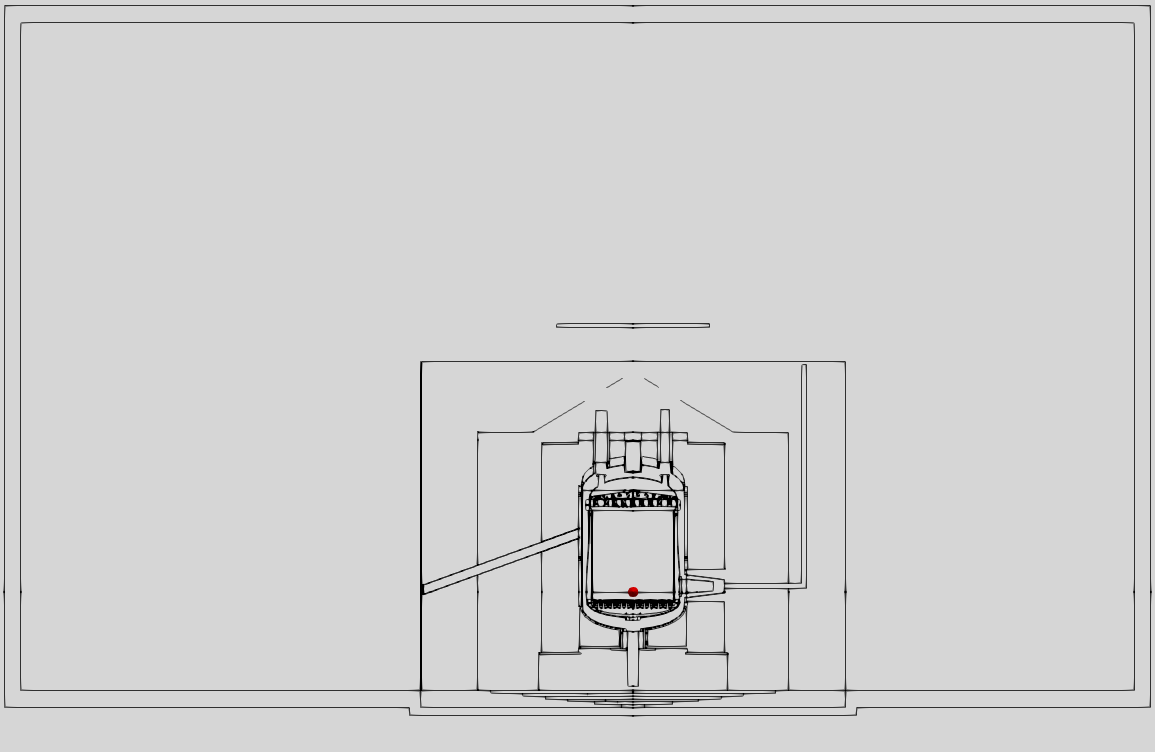
\includegraphics[width=\textwidth]{Figures/Simulations/cavern_geometry_2.png}
\centering
\caption{LZ detector geometry slice with additional cavern geometry. OD PMTs are not seen present as they do not lie in this plane.}
\label{fig:Cavern_Geometry}
\end{figure}

\par
The generator uses biasing etc... blah blah blah


\par
This generator however did not include anything below 2MeV, resulting in $^{40}K$ not being included at all and the resultant expected rates being lower than expected.
Additionally it was noticed that in the previous generator the distribution was not a cylinder but rather a table.
The result of this would be that the $\gamma$ distribution is biased to the top and bottom of the detectors more so than it would otherwise be.
This is highlighted in Figures \ref{fig:cavern_gamma_energy_distribution} and \ref{fig:cavern_gamma_position_distribution}.


\begin{figure}[!htbp]%
\centering
\begin{tikzpicture}
\centering
    \begin{groupplot}[%view={0}{90},
    group style = {group size = 2 by 1}]
    \nextgroupplot[
            xlabel=Energy (keV),
            ylabel=Rate (Hz/15keV),
            width=0.5\textwidth, height=6cm,
            xmin=0, xmax=14000,
            minor y tick num=4,
            ymode=log, ymin=1e-6, ymax=10,
            grid=major,]
            \addplot[green, mark=none]
                    table [x=Bins,y=Weights]
                    {Data/Simulation_Analysis/Cavern_Gammas/old_gamma_generator_th232.dat};
            \addplot[blue, mark=none]
                    table [x=Bins,y=Weights]
                    {Data/Simulation_Analysis/Cavern_Gammas/old_gamma_generator_u238.dat};

        \nextgroupplot[
            xlabel=Energy (keV),
            width=0.5\textwidth, height=6cm,
            xmin=0, xmax=14000,
            yticklabel pos=right,
            minor y tick num=4,
            ymode=log, ymin=1e-6, ymax=10,
            grid=major,
            legend style = { column sep = 10pt, legend columns = -1, legend to name = Cavern_Gamma_CommonLegend,}]
            \addplot[green, mark=none]
                    table [x=Bins,y=Weights]
                    {Data/Simulation_Analysis/Cavern_Gammas/new_gamma_generator_th232.dat};
            \addplot[blue, mark=none]
                    table [x=Bins,y=Weights]
                    {Data/Simulation_Analysis/Cavern_Gammas/new_gamma_generator_u238.dat};
            \addplot[red, mark=none]
                    table [x=Bins,y=Weights]
                    {Data/Simulation_Analysis/Cavern_Gammas/new_gamma_generator_k40.dat};
            \legend{${}^{232}Th$, ${}^{238}U$, ${}^{40}K$}
            
    \end{groupplot}
    \node at ($(group c2r1) - (group c1r1) + (-0.5cm, 5.0cm)$) {\ref{Cavern_Gamma_CommonLegend}};
\end{tikzpicture}
\caption{Generator $\gamma$ energies. \textbf{Left:} Previous generator. \textbf{Right:} newly created generator.}
\label{fig:cavern_gamma_energy_distribution}
\end{figure}



\begin{figure}[!htbp]
    \centering
    
\includegraphics[width=0.5\textwidth]{Figures/Placeholder.png}
    \caption{Simulated cavern $\gamma$ energy deposit locations in the OD normalised to rates from \cite{LZ_Gamma_Ray_Background_ref}. \textbf{Left:} Previous generator. \textbf{Right:} newly created generator.}
    \label{fig:cavern_gamma_position_distribution}
\end{figure}


\par


\begin{figure}[!htbp]
    \centering
    
\includegraphics[width=0.5\textwidth]{Figures/Placeholder.png}
    \caption{Change in OD rate between different generator versions}
    \label{fig:cavern_gamma_rate_difference}
\end{figure}



\begin{table}[!htbp]
    \centering
    \begin{tabular}{c|c|c|c}
        Generator    & Activity (Bq/kg) & Boost per surface & Generator livetime   \\ \hline
        ${}^{40}K$   & 216              & 28                & 57.72                \\
        ${}^{238}U$  & 29.1             & 34                & 60.26                \\
        ${}^{232}Th$ & 12.5             & 70                & 60.66
    \end{tabular}
    \caption{Parameters used in generator creation. Activity rates are from \cite{LZ_Gamma_Ray_Background_ref}.}
    \label{tab:cavern_gamma_generator_parameters}
\end{table}

\par
The livetime for each $\gamma$ can be determined then by $l = \frac{n. \gamma simulated}{n. \gamma in generator} * generator livetime$

\par
In short, this means that every $\gamma$ in the generator represents 130000 decays from the rock, and so is a significant computational saving.